\section*{Question 3}
\begin{figure}[h]
    \centering
    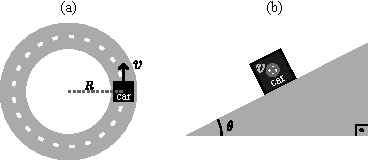
\includegraphics[width=0.65\textwidth]{figures/q3.pdf}
    \label{fig:q4}
\end{figure}
\noindent
A car of mass $m$ is moving at a speed $v$ around a curve with a radius $R$. The coefficient of static friction between the tires and the road is $\mu_s$, and the gravitational acceleration is $g$.

\begin{itemize}
    \item [(a)] Determine the maximum speed $v_{\text{max}}$ at which the car can navigate the curve safely to avoid slippage as shown in Figure (a). --- \textit{0.7 points}
    
    \item [(b)] If the road is banked as shown in Figure (b) at an angle $\theta$ with respect to the horizontal, find the maximum speed for which the car can take the curved path safely \underline{without depending on friction}. --- \textit{0.3 points}
\end{itemize}
\underline{Note}: All the other other external forces, such as air resistance, are negligible.

\section*{Solution:}